% Options for packages loaded elsewhere
\PassOptionsToPackage{unicode}{hyperref}
\PassOptionsToPackage{hyphens}{url}
%
\documentclass[
]{article}
\usepackage{lmodern}
\usepackage{amssymb,amsmath}
\usepackage{ifxetex,ifluatex}
\ifnum 0\ifxetex 1\fi\ifluatex 1\fi=0 % if pdftex
  \usepackage[T1]{fontenc}
  \usepackage[utf8]{inputenc}
  \usepackage{textcomp} % provide euro and other symbols
\else % if luatex or xetex
  \usepackage{unicode-math}
  \defaultfontfeatures{Scale=MatchLowercase}
  \defaultfontfeatures[\rmfamily]{Ligatures=TeX,Scale=1}
\fi
% Use upquote if available, for straight quotes in verbatim environments
\IfFileExists{upquote.sty}{\usepackage{upquote}}{}
\IfFileExists{microtype.sty}{% use microtype if available
  \usepackage[]{microtype}
  \UseMicrotypeSet[protrusion]{basicmath} % disable protrusion for tt fonts
}{}
\makeatletter
\@ifundefined{KOMAClassName}{% if non-KOMA class
  \IfFileExists{parskip.sty}{%
    \usepackage{parskip}
  }{% else
    \setlength{\parindent}{0pt}
    \setlength{\parskip}{6pt plus 2pt minus 1pt}}
}{% if KOMA class
  \KOMAoptions{parskip=half}}
\makeatother
\usepackage{xcolor}
\IfFileExists{xurl.sty}{\usepackage{xurl}}{} % add URL line breaks if available
\IfFileExists{bookmark.sty}{\usepackage{bookmark}}{\usepackage{hyperref}}
\hypersetup{
  hidelinks,
  pdfcreator={LaTeX via pandoc}}
\urlstyle{same} % disable monospaced font for URLs
\usepackage{color}
\usepackage{fancyvrb}
\newcommand{\VerbBar}{|}
\newcommand{\VERB}{\Verb[commandchars=\\\{\}]}
\DefineVerbatimEnvironment{Highlighting}{Verbatim}{commandchars=\\\{\}}
% Add ',fontsize=\small' for more characters per line
\newenvironment{Shaded}{}{}
\newcommand{\AlertTok}[1]{\textcolor[rgb]{1.00,0.00,0.00}{\textbf{#1}}}
\newcommand{\AnnotationTok}[1]{\textcolor[rgb]{0.38,0.63,0.69}{\textbf{\textit{#1}}}}
\newcommand{\AttributeTok}[1]{\textcolor[rgb]{0.49,0.56,0.16}{#1}}
\newcommand{\BaseNTok}[1]{\textcolor[rgb]{0.25,0.63,0.44}{#1}}
\newcommand{\BuiltInTok}[1]{#1}
\newcommand{\CharTok}[1]{\textcolor[rgb]{0.25,0.44,0.63}{#1}}
\newcommand{\CommentTok}[1]{\textcolor[rgb]{0.38,0.63,0.69}{\textit{#1}}}
\newcommand{\CommentVarTok}[1]{\textcolor[rgb]{0.38,0.63,0.69}{\textbf{\textit{#1}}}}
\newcommand{\ConstantTok}[1]{\textcolor[rgb]{0.53,0.00,0.00}{#1}}
\newcommand{\ControlFlowTok}[1]{\textcolor[rgb]{0.00,0.44,0.13}{\textbf{#1}}}
\newcommand{\DataTypeTok}[1]{\textcolor[rgb]{0.56,0.13,0.00}{#1}}
\newcommand{\DecValTok}[1]{\textcolor[rgb]{0.25,0.63,0.44}{#1}}
\newcommand{\DocumentationTok}[1]{\textcolor[rgb]{0.73,0.13,0.13}{\textit{#1}}}
\newcommand{\ErrorTok}[1]{\textcolor[rgb]{1.00,0.00,0.00}{\textbf{#1}}}
\newcommand{\ExtensionTok}[1]{#1}
\newcommand{\FloatTok}[1]{\textcolor[rgb]{0.25,0.63,0.44}{#1}}
\newcommand{\FunctionTok}[1]{\textcolor[rgb]{0.02,0.16,0.49}{#1}}
\newcommand{\ImportTok}[1]{#1}
\newcommand{\InformationTok}[1]{\textcolor[rgb]{0.38,0.63,0.69}{\textbf{\textit{#1}}}}
\newcommand{\KeywordTok}[1]{\textcolor[rgb]{0.00,0.44,0.13}{\textbf{#1}}}
\newcommand{\NormalTok}[1]{#1}
\newcommand{\OperatorTok}[1]{\textcolor[rgb]{0.40,0.40,0.40}{#1}}
\newcommand{\OtherTok}[1]{\textcolor[rgb]{0.00,0.44,0.13}{#1}}
\newcommand{\PreprocessorTok}[1]{\textcolor[rgb]{0.74,0.48,0.00}{#1}}
\newcommand{\RegionMarkerTok}[1]{#1}
\newcommand{\SpecialCharTok}[1]{\textcolor[rgb]{0.25,0.44,0.63}{#1}}
\newcommand{\SpecialStringTok}[1]{\textcolor[rgb]{0.73,0.40,0.53}{#1}}
\newcommand{\StringTok}[1]{\textcolor[rgb]{0.25,0.44,0.63}{#1}}
\newcommand{\VariableTok}[1]{\textcolor[rgb]{0.10,0.09,0.49}{#1}}
\newcommand{\VerbatimStringTok}[1]{\textcolor[rgb]{0.25,0.44,0.63}{#1}}
\newcommand{\WarningTok}[1]{\textcolor[rgb]{0.38,0.63,0.69}{\textbf{\textit{#1}}}}
\usepackage{graphicx,grffile}
\makeatletter
\def\maxwidth{\ifdim\Gin@nat@width>\linewidth\linewidth\else\Gin@nat@width\fi}
\def\maxheight{\ifdim\Gin@nat@height>\textheight\textheight\else\Gin@nat@height\fi}
\makeatother
% Scale images if necessary, so that they will not overflow the page
% margins by default, and it is still possible to overwrite the defaults
% using explicit options in \includegraphics[width, height, ...]{}
\setkeys{Gin}{width=\maxwidth,height=\maxheight,keepaspectratio}
% Set default figure placement to htbp
\makeatletter
\def\fps@figure{htbp}
\makeatother
\setlength{\emergencystretch}{3em} % prevent overfull lines
\providecommand{\tightlist}{%
  \setlength{\itemsep}{0pt}\setlength{\parskip}{0pt}}
\setcounter{secnumdepth}{-\maxdimen} % remove section numbering

\date{}

\begin{document}

\hypertarget{header-n2}{%
\section{Nov 12 Tue}\label{header-n2}}

\begin{quote}
絕望的星期二
\end{quote}

\hypertarget{header-n5}{%
\subsection{SE-302::Compilers}\label{header-n5}}

今天要講的內容是 Global Optimization。全局性的優化。

\hypertarget{header-n7}{%
\subsubsection{Flow Analysis}\label{header-n7}}

對全局的控制流進行分析,觀察是否有什麼可以刪除的 Code。

先看局部的情形。

\hypertarget{header-n10}{%
\paragraph{Local Optimization}\label{header-n10}}

The simple optimizations in basic blocks are:

\begin{itemize}
\item
  Constant propagation
\item
  Dead code elimination
\end{itemize}

如臨時變量的常數指派就可以被安全地刪除:

\begin{verbatim}
X := 3
Y := Z * W
Q := X + Y

=>

X := 3
Y := Z * W
Q := 3 + Y

=>

Y := Z * W
Q := 3 + Y
\end{verbatim}

如是。

\hypertarget{header-n20}{%
\paragraph{Goes to Global}\label{header-n20}}

到了全局就比較複雜了;如果要做一個點的優化,會影響到全局所有變量、所有路徑。都會產生干涉。

如何確定我們的優化的「正確性」呢?這是我們最關心的。

\hypertarget{header-n23}{%
\paragraph{Correctness}\label{header-n23}}

我們把所有變元分為兩類:Live or Dead。

Live: 可能在其後被用到的(Might be used)

Dead: 不可能在其後被用到的(Never be used)

留意:Live 只是可能被用到,我們就不能刪掉它。只有完全確定不可能被用到的
Dead 才能被安全地優化掉。

\hypertarget{header-n28}{%
\paragraph{Liveness}\label{header-n28}}

判斷一個變量:他是活著的嗎?

我們有這樣一套判據:

A variable \(x\) is live at statement \(s\) if

\begin{itemize}
\item
  There exists a statement \(s’\) that uses \(x\)
\item
  There is a path from \(s\) to \(s’\)
\item
  That path has no intervening assignment to \(x\)
\end{itemize}

好像很有道理:如果 \(s\) 有到 \(s'\) 的通路(或者乾脆就是他自己),在
\(s'\) 處用到了 \(x\),且這條通路之間沒有介入對 \(x\) 的賦值,則稱 \(x\)
在 \(s\) 中是活的。

\hypertarget{header-n40}{%
\subsubsection{Global Analysis}\label{header-n40}}

Global optimization tasks share several traits:

\begin{itemize}
\item
  The optimization depends on knowing a property \(X\) at a particular
  point in program execution
\item
  Proving \(X\) at any point requires knowledge of the entire function
  body
\item
  It is OK to be conservative. If the optimization requires \(X\) to be
  true, then want to know either

  \begin{itemize}
  \item
    \(X\) is definitely true
  \item
    Don't know if \(X\) is true
  \end{itemize}
\item
  It is always safe to say ``don't know''
\end{itemize}

總歸,要判斷任何位置的 \(X\) 都需要全局的信息才能確定。

如果你不能確定,那麼就走保守路線,在優化的時候 Being Conservative
不會錯。

\hypertarget{header-n58}{%
\paragraph{Rules}\label{header-n58}}

\hypertarget{header-n59}{%
\subparagraph{規則一}\label{header-n59}}

\begin{figure}
\centering
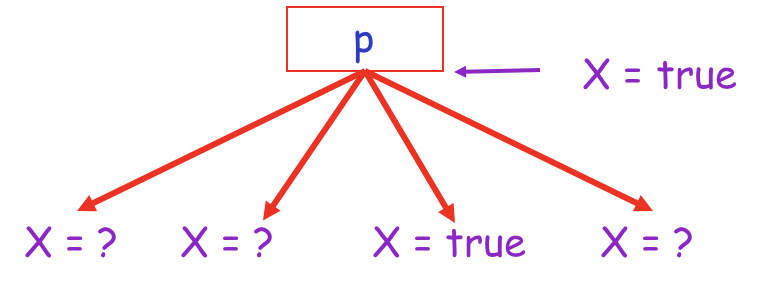
\includegraphics{/Users/yue/Documents/GitHub/2019-2020-autumn-semester/11-november/12.assets/image-20191112083430243.png}
\caption{}
\end{figure}

\begin{figure}
\centering
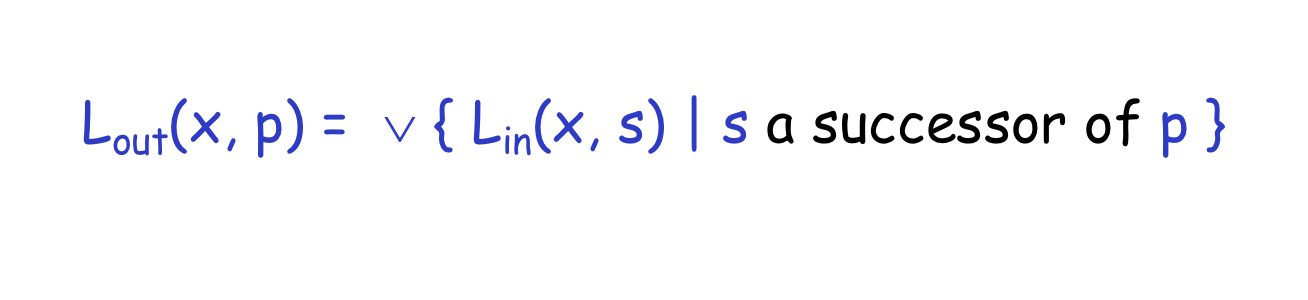
\includegraphics{/Users/yue/Documents/GitHub/2019-2020-autumn-semester/11-november/12.assets/image-20191112083438535.png}
\caption{}
\end{figure}

\hypertarget{header-n62}{%
\subparagraph{規則二}\label{header-n62}}

\begin{figure}
\centering
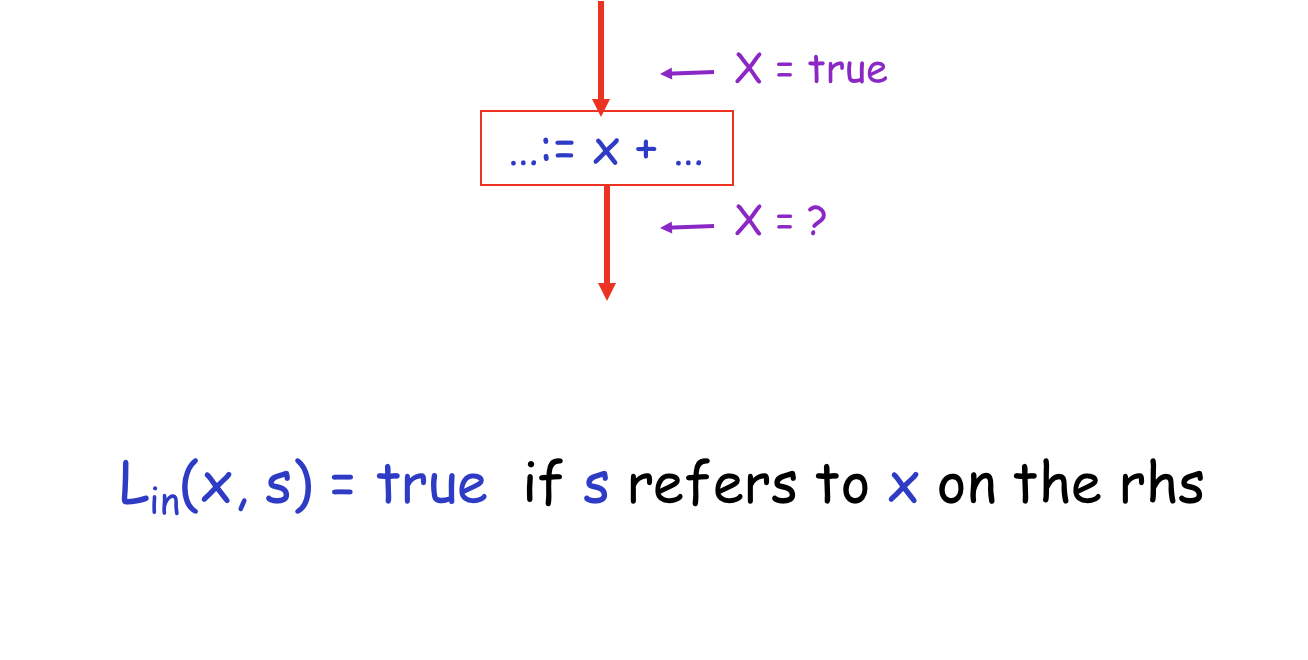
\includegraphics{/Users/yue/Documents/GitHub/2019-2020-autumn-semester/11-november/12.assets/image-20191112083450752.png}
\caption{}
\end{figure}

這種賦值,新值跟原值是有關係的。因此是有作用的。不能視為死的。

\hypertarget{header-n65}{%
\subparagraph{規則三}\label{header-n65}}

\begin{figure}
\centering
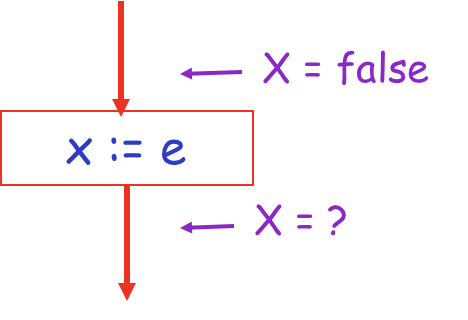
\includegraphics{/Users/yue/Documents/GitHub/2019-2020-autumn-semester/11-november/12.assets/image-20191112083541755.png}
\caption{}
\end{figure}

假若 \(e\) 沒有利用到 \(x\),那就不算他活著。

\hypertarget{header-n68}{%
\subparagraph{規則四}\label{header-n68}}

\begin{figure}
\centering
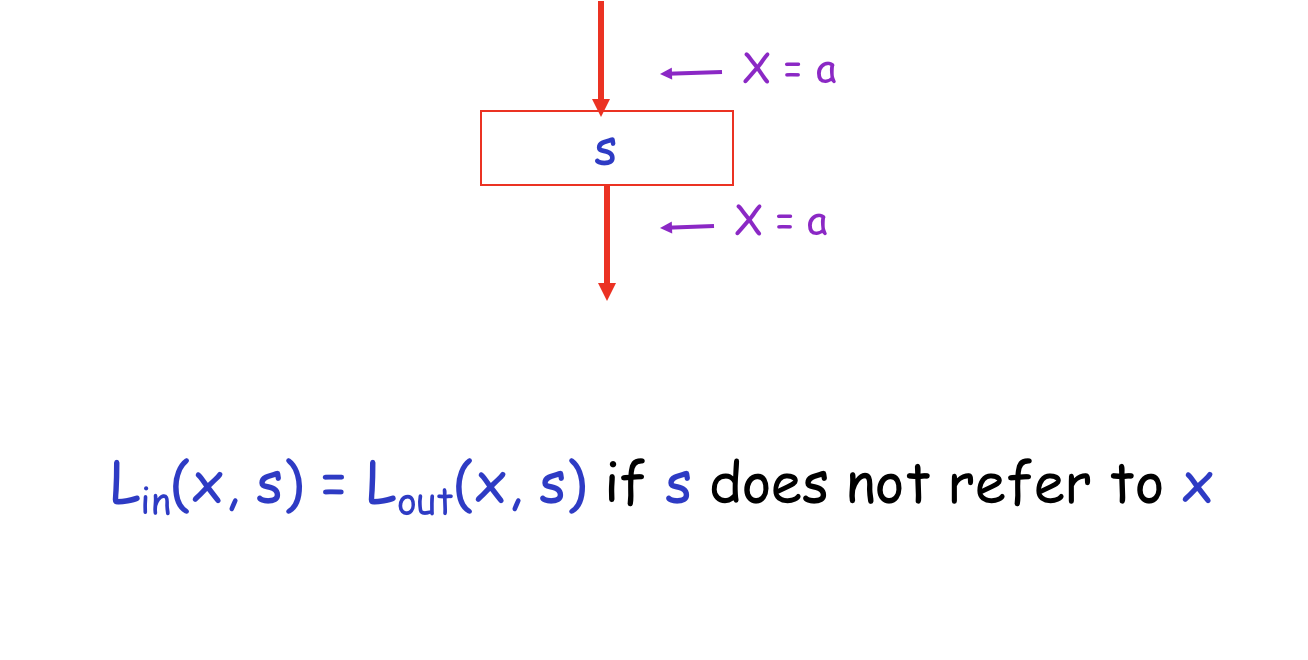
\includegraphics{/Users/yue/Documents/GitHub/2019-2020-autumn-semester/11-november/12.assets/image-20191112083617635.png}
\caption{}
\end{figure}

\hypertarget{header-n70}{%
\paragraph{Algorithms}\label{header-n70}}

\begin{enumerate}
\def\labelenumi{\arabic{enumi}.}
\item
  Let all L\_(\ldots) = false initially
\item
  Repeat until all statements s satisfy rules 1 - 4

  Pick s where one of 1 - 4 does not hold and update using the
  appropriate rule.
\end{enumerate}

一開始把所有人都認定為 False。然後重複利用規則 1 到規則
4,重複對整體進行 True 化,直到沒有可以繼續執行的部分。

\begin{figure}
\centering
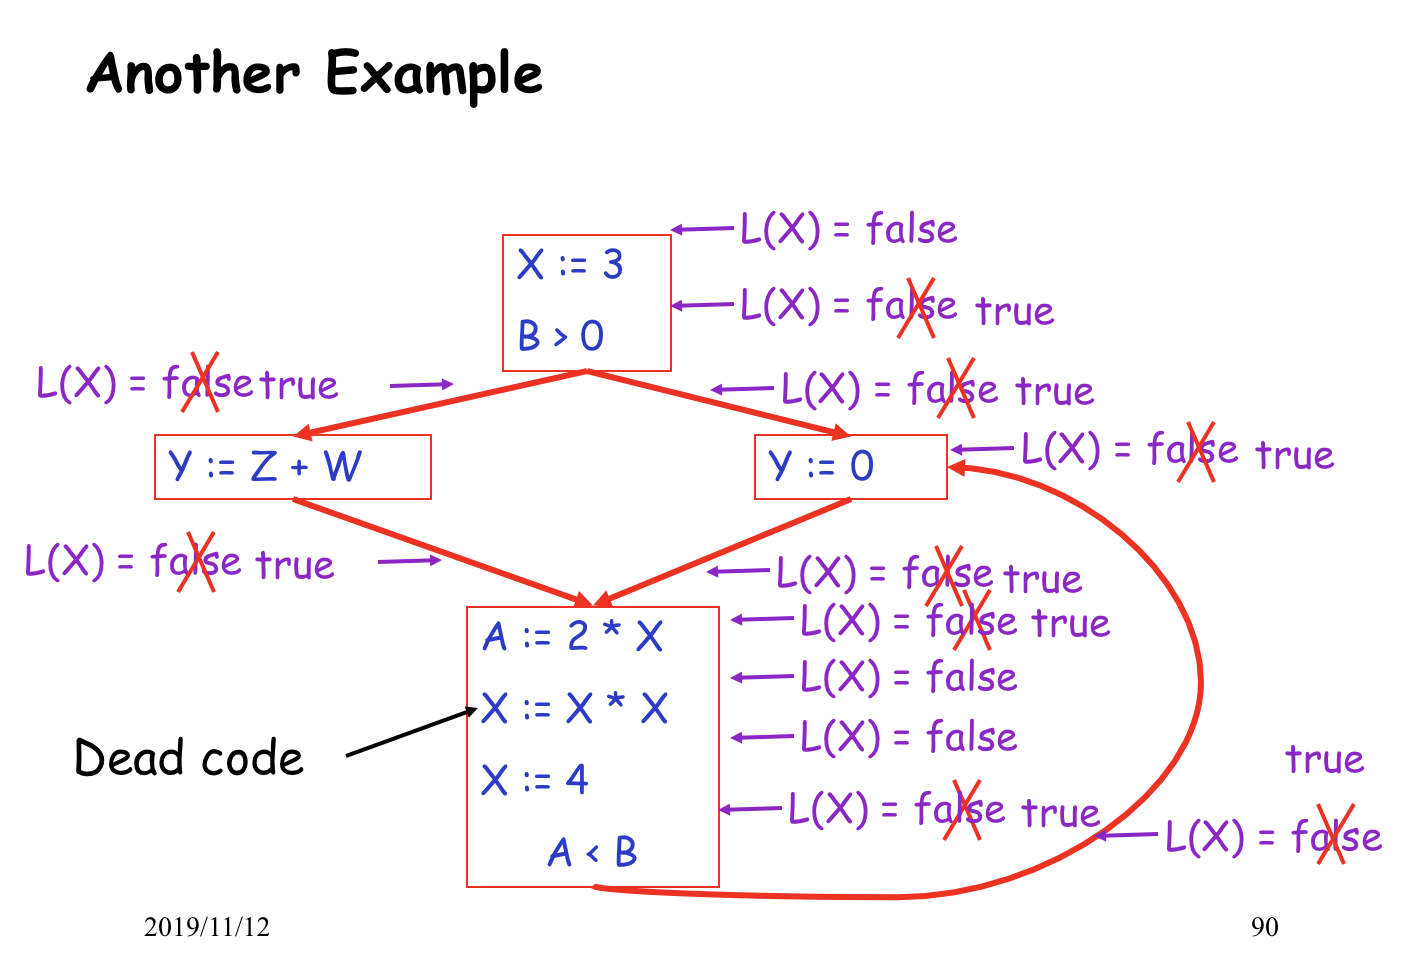
\includegraphics{/Users/yue/Documents/GitHub/2019-2020-autumn-semester/11-november/12.assets/image-20191112084205270.png}
\caption{}
\end{figure}

總歸,整個過程就是不斷利用四個規則將 False 改寫成 True 的過程。

\hypertarget{header-n80}{%
\paragraph{Computing Liveness Set}\label{header-n80}}

現在我們已經分析出了每個位置的 Liveness 性;那麼接下來我們該拿這個 True
/ False 集合怎麼辦呢?

\hypertarget{header-n82}{%
\paragraph{Termination}\label{header-n82}}

\begin{itemize}
\item
  A value can change from false to true, but not the other way around
\end{itemize}

註:一個變量從 False 變成 True 之後,就不可能再從 True 變回到 False 了。

\begin{itemize}
\item
  Each value can change only once, so termination is guaranteed
\end{itemize}

由上條可知,每一個值最多只可能變換一次。因此不會不停地變下去。

\begin{itemize}
\item
  Once the analysis is computed, it is simple to eliminate dead code
\end{itemize}

一旦所有的「轉換分析」結束,就很容易分析死代碼了。

\hypertarget{header-n95}{%
\paragraph{Example}\label{header-n95}}

\begin{figure}
\centering
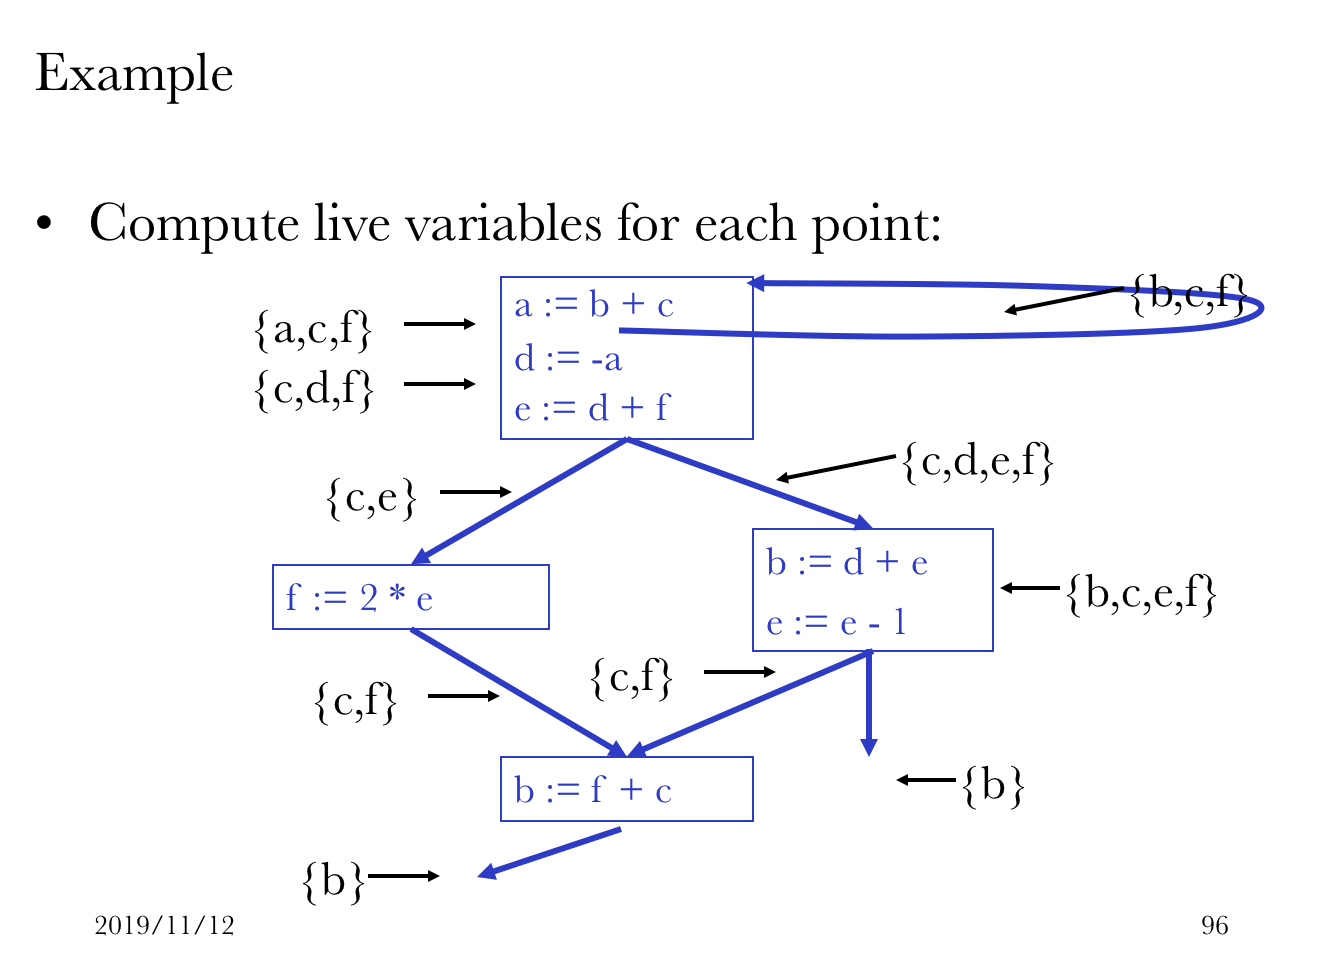
\includegraphics{/Users/yue/Documents/GitHub/2019-2020-autumn-semester/11-november/12.assets/image-20191112092105223.png}
\caption{}
\end{figure}

\hypertarget{header-n97}{%
\subsubsection{Termination}\label{header-n97}}

\hypertarget{header-n98}{%
\paragraph{When?}\label{header-n98}}

Simply saying ``repeat until nothing changes'' doesn't guarantee that
eventually nothing changes.

\hypertarget{header-n100}{%
\subsubsection{Register Allocation}\label{header-n100}}

\hypertarget{header-n101}{%
\paragraph{Main Idea}\label{header-n101}}

之前生成代碼的時候,從來都是隨便用寄存器的。一分錢不花,想加多少加多少。

\hypertarget{header-n103}{%
\paragraph{Interference Graph}\label{header-n103}}

\begin{itemize}
\item
  Step 1 (build): build an Interference graph

  \begin{itemize}
  \item
    Nodes of the graph = variables
  \item
    Edges connect variables that interfere with one another
  \end{itemize}
\item
  Nodes will be assigned a color corresponding to the register assigned
  to the variable
\item
  Two nodes with the same color can't be next to one another in the
  graph
\end{itemize}

\hypertarget{header-n116}{%
\subsection{SE-227::CSE}\label{header-n116}}

上節課講過了 Lock
的實現。可以軟件實現也可以硬件實現;但軟件實現總是不靠譜的。(如底層硬件用了弱化版的
Cache Consistency 的話,那鎖就不牢靠了。)

總歸還是硬件實現的最靠譜;如果沒按實際情況來你可以去找 Intel/AMD
退錢(×)

\hypertarget{header-n119}{%
\subsubsection{Thread \& Condition Variable}\label{header-n119}}

\hypertarget{header-n120}{%
\paragraph{Buffer API}\label{header-n120}}

\begin{itemize}
\item
  Bounded buffer: a buffer that stores (up to) N messages
\item
  Bounded buffer API

  send (m)

  m \textless- receive()
\end{itemize}

API 設計很簡單;直接 call \texttt{send} 跟 \texttt{receive} 就能實現
Buffer 交換了。

\hypertarget{header-n129}{%
\paragraph{SEND \& RECEIVE}\label{header-n129}}

留意到 Send 和 Receive 都是 System Call 級別的。

\begin{itemize}
\item
  Supervisor calls (e.g., system calls)
\item
  Copy the message from/to the thread's domain to/from the shared buffer
\item
  Programs running in kernel mode is written carefully
\item
  Transitions between user mode and kernel mode can be expensive
\end{itemize}

\hypertarget{header-n140}{%
\paragraph{Bounded Buffer Send}\label{header-n140}}

\begin{figure}
\centering
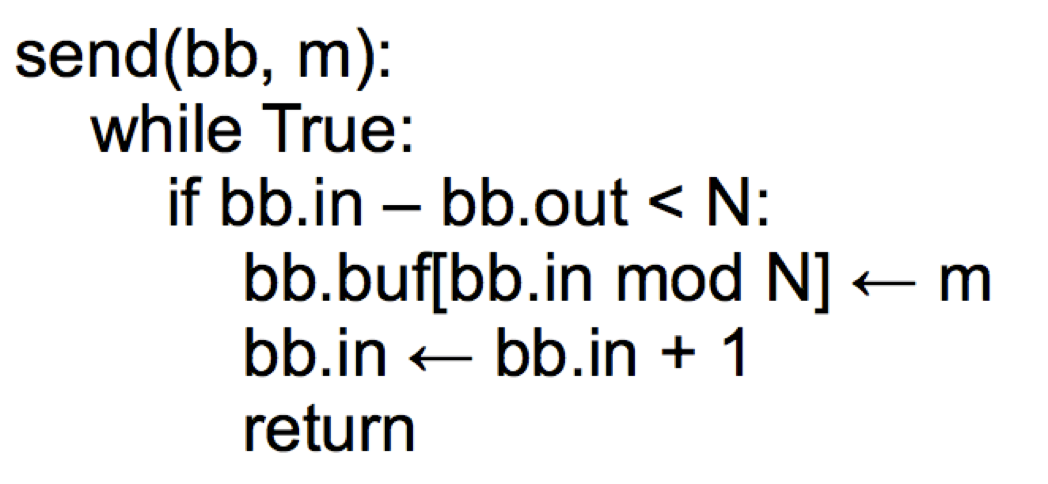
\includegraphics{/Users/yue/Documents/GitHub/2019-2020-autumn-semester/11-november/12.assets/image-20191112101238882.png}
\caption{}
\end{figure}

Send 的實現如上所述;旁註特別說明不可以交換雙向箭頭所指的兩行語句。

原因是什麼?

\begin{figure}
\centering
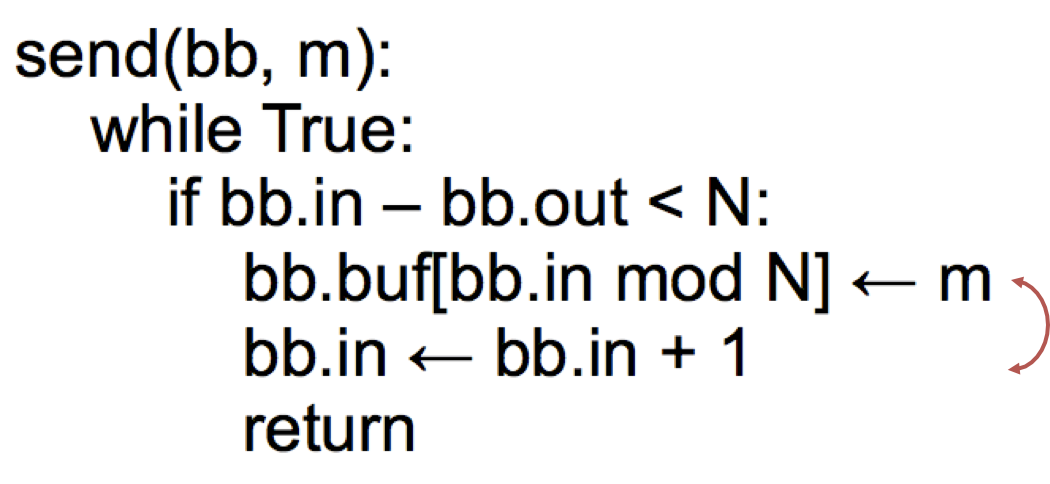
\includegraphics{/Users/yue/Documents/GitHub/2019-2020-autumn-semester/11-november/12.assets/image-20191112101547279.png}
\caption{}
\end{figure}

如果我們先 + 1 再放置 Buffer Value,那麼就可以直接 Call Receive
了。然而此時值還沒進去!

假如在這兩條語句之間 Receive 被
call,那麼就等於是讀到了垃圾值。這不應該。

Before or After 告訴我們不能把錯誤的中間狀態暴露給別人。

所以,先放值再廣播說「喜+1」,而非反過來。

\hypertarget{header-n149}{%
\paragraph{Lock Myth}\label{header-n149}}

我們之前不是說,所有的多線程操作都得加鎖嗎。這裡怎麼沒有鎖,實現居然也可以用?

因為我們這個算法只能被用在 One Sender \& One Receiver 的情況。

如果有兩個 Sender 或是兩個 Receiver,就會同時遞增/遞減
bb.in,這肯定會有問題。

但是,這裏在 Single Producer \& Single Consumer 的情況下是可以用的。

\hypertarget{header-n154}{%
\paragraph{Bounded Buffer Send \& Receive}\label{header-n154}}

\begin{figure}
\centering
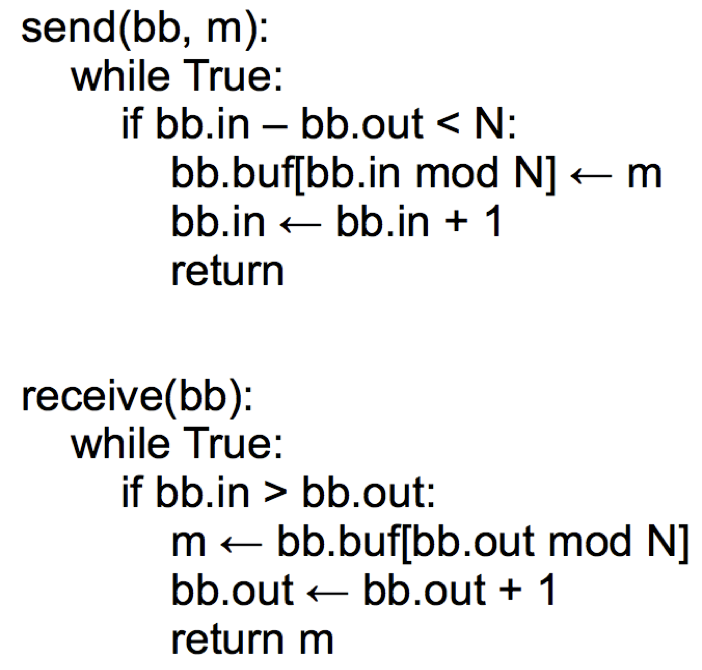
\includegraphics{/Users/yue/Documents/GitHub/2019-2020-autumn-semester/11-november/12.assets/image-20191112101913926.png}
\caption{}
\end{figure}

同樣的,有下面的 Assumption:

\begin{enumerate}
\def\labelenumi{\arabic{enumi}.}
\item
  Single producer \& Single consumer 
\item
  Each on its own CPU
\item
  in and out do not overflow 
\item
  read/write coherence (e.g., on cache)
\item
  in and out ensure before-or-after atomicity
\item
  The result of executing a statement becomes visible to other threads
  in program order

  \begin{itemize}
  \item
    Compilers cannot optimize it
  \end{itemize}
\end{enumerate}

\hypertarget{header-n173}{%
\subsubsection{Lockerize}\label{header-n173}}

現在我們希望我們的 Send / Receive 程序可以運行在多個 CPU
上,可以支持多個 Sender 和 Receiver。

因此我們得加鎖。

\hypertarget{header-n176}{%
\paragraph{Wrong Version}\label{header-n176}}

\begin{figure}
\centering
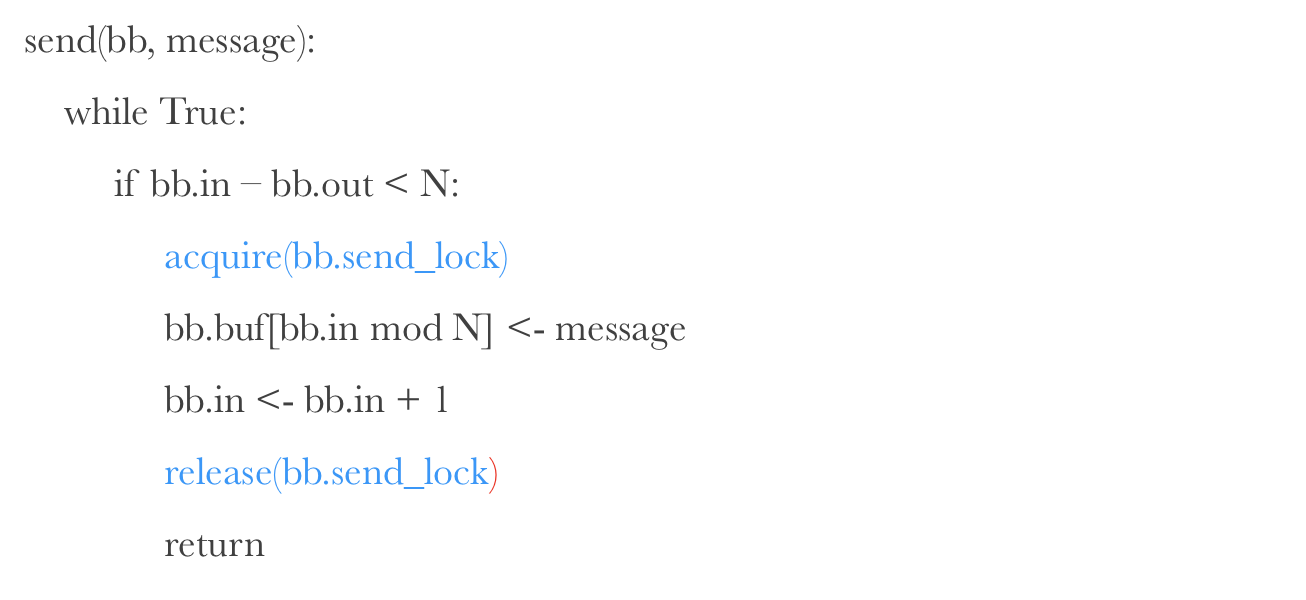
\includegraphics{/Users/yue/Documents/GitHub/2019-2020-autumn-semester/11-november/12.assets/image-20191112102559227.png}
\caption{}
\end{figure}

這個算法的問題在於:if bb.in - bb.out 條件沒被加鎖,因此可能有多個
Sender 同時被允許進入 acquire 中,可是其實這時候可能已經沒有足夠的空間給
Send 了。(錯誤判斷形勢的原因是髒讀了 bb.in - bb.out。)

\hypertarget{header-n179}{%
\paragraph{Right Version}\label{header-n179}}

\begin{figure}
\centering
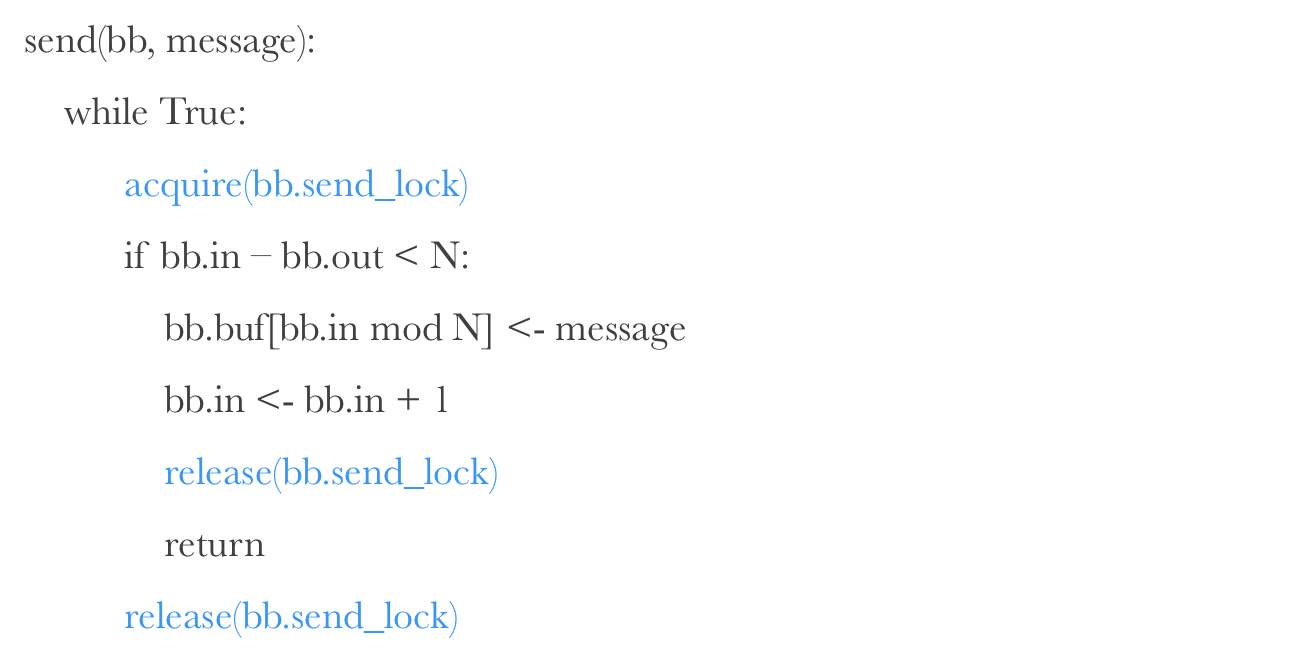
\includegraphics{/Users/yue/Documents/GitHub/2019-2020-autumn-semester/11-november/12.assets/image-20191112102843136.png}
\caption{}
\end{figure}

這個版本裡進去就先拿鎖;假如空間不夠(bb.in - bb.out \textgreater=
N),就直接放棄鎖。

\hypertarget{header-n182}{%
\subsubsection{\texorpdfstring{\texttt{yield()}}{yield()}}\label{header-n182}}

何謂 yield?

\begin{itemize}
\item
  When using locking, current thread is busy waiting for an event
\item
  Implementation of yield():
\end{itemize}

\begin{enumerate}
\def\labelenumi{\arabic{enumi}.}
\item
  Suspend running thread: save stack pointer and page-table register
\item
  Choose new thread: round-robin fashion until we hit a RUNNABLE thread
  (perhaps the one that just called yield)
\item
  Resume thread to run: reload state all of this happens as an atomic
  action
\end{enumerate}

\begin{itemize}
\item
  Data structures

  \begin{itemize}
  \item
    threads table, CPUs table, t\_lock
  \end{itemize}
\end{itemize}

\hypertarget{header-n202}{%
\paragraph{Appliance}\label{header-n202}}

您在 yield 的時候,切莫拿著鎖做這個操作。否則就鎖死了。

\hypertarget{header-n204}{%
\paragraph{Implementation}\label{header-n204}}

yield 是怎麼實現的呢?主要分三步走:

\begin{Shaded}
\begin{Highlighting}[]
\CommentTok{// Suspend the running thread}

\CommentTok{// Choose a new thread}

\CommentTok{// Resume the new thread}
\end{Highlighting}
\end{Shaded}

\hypertarget{header-n207}{%
\subparagraph{Suspend the Running Thread}\label{header-n207}}

\begin{Shaded}
\begin{Highlighting}[]
\NormalTok{yield():}
\NormalTok{  acquire(t_lock)}

\NormalTok{  id = id of current thread}
\NormalTok{  threads[id].state = RUNNABLE}
\NormalTok{  threads[id].sp = SP}

  \CommentTok{// Choose a new thread}
  \CommentTok{// Resume the new thread}
  
\NormalTok{  release(t_lock)}
\end{Highlighting}
\end{Shaded}

\begin{figure}
\centering
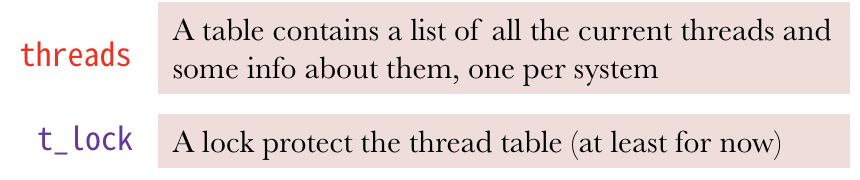
\includegraphics{/Users/yue/Documents/GitHub/2019-2020-autumn-semester/11-november/12.assets/image-20191112103835803.png}
\caption{}
\end{figure}

\hypertarget{header-n210}{%
\subparagraph{Choose a New Thread}\label{header-n210}}

\begin{figure}
\centering
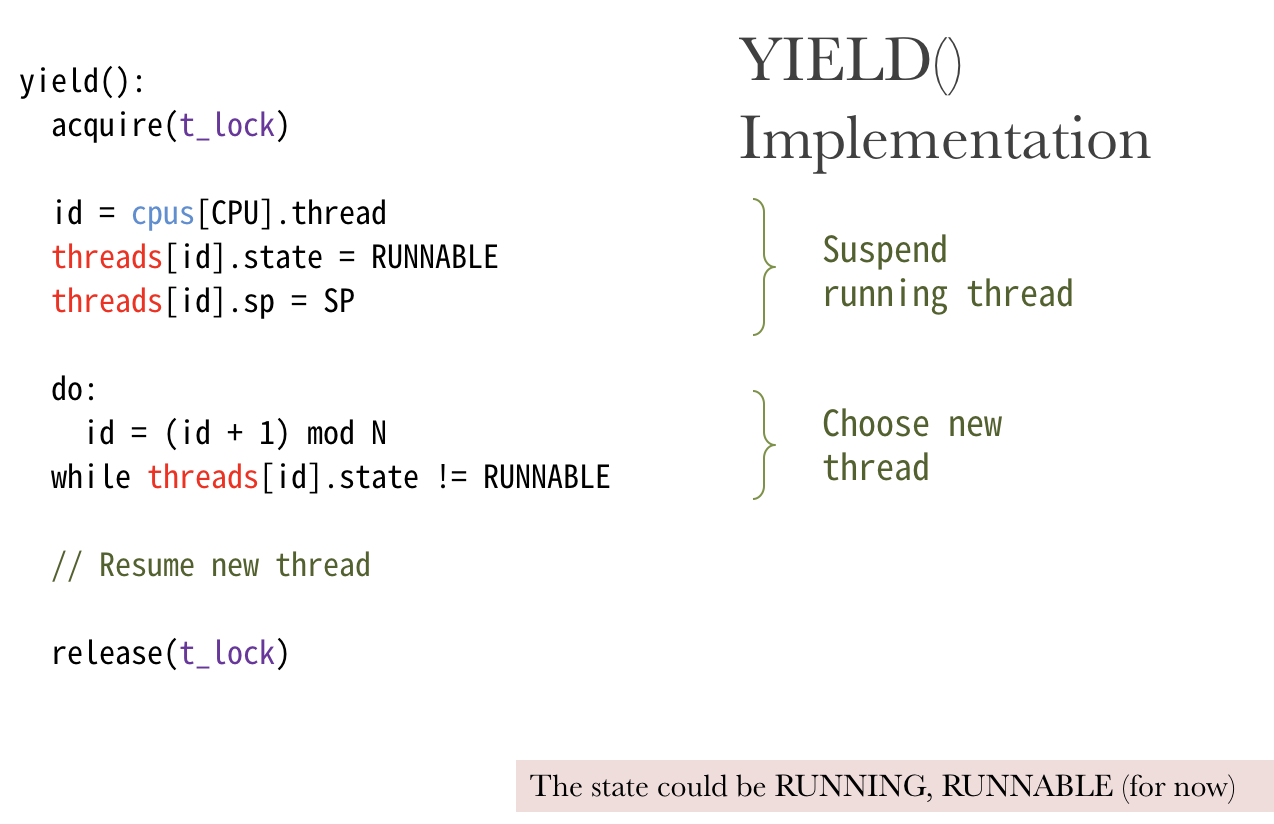
\includegraphics{/Users/yue/Documents/GitHub/2019-2020-autumn-semester/11-november/12.assets/image-20191112103914691.png}
\caption{}
\end{figure}

\hypertarget{header-n212}{%
\subparagraph{Resume New Thread}\label{header-n212}}

\begin{figure}
\centering
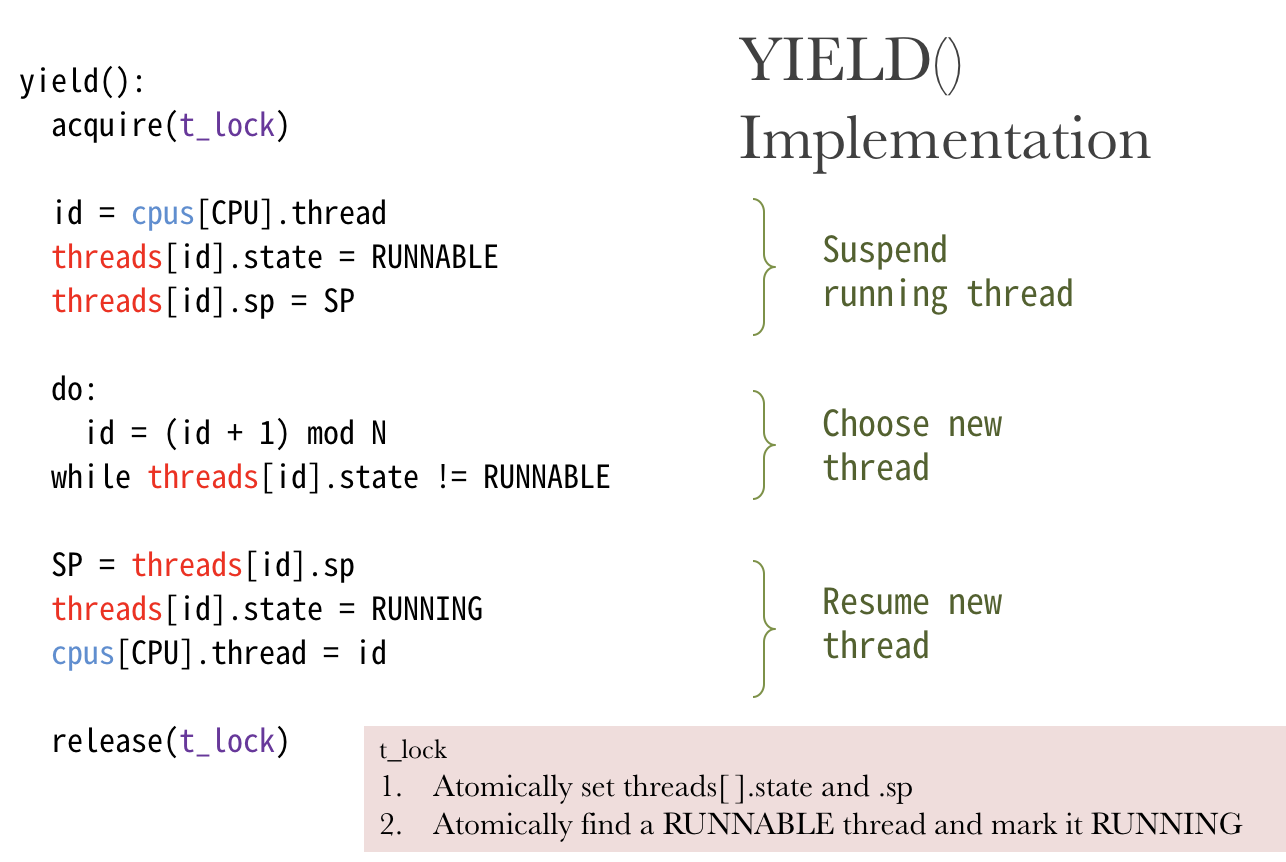
\includegraphics{/Users/yue/Documents/GitHub/2019-2020-autumn-semester/11-november/12.assets/image-20191112103923875.png}
\caption{}
\end{figure}

\hypertarget{header-n214}{%
\subsubsection{Conditional Variables}\label{header-n214}}

Yield 的問題就在於造成了 a lot of unnecessary checking as well as a lot
of acquiring locks。

更好的解決方案:不要一次把所有人都叫一遍,不如 the sender (receiver)
just got woken up when the buffer is not full (empty)。

\hypertarget{header-n217}{%
\paragraph{Definition}\label{header-n217}}

\begin{itemize}
\item
  Condition Variable

  \begin{itemize}
  \item
    Let threads wait for events
  \item
    The threads get notified when the events occur
  \end{itemize}
\item
  Condition variable API

  \begin{itemize}
  \item
    WAIT(cv): yield processor and wait to be notified of cv
  \item
    NOTIFY(cv): notify waiting threads of cv
  \end{itemize}
\end{itemize}

\end{document}
